% Pengaturan ukuran teks dan bentuk halaman dua sisi
\documentclass[12pt]{book}

% Pengaturan ukuran halaman dan margin
\usepackage[a4paper,top=30mm,left=30mm,right=20mm,bottom=25mm]{geometry}

% Pengaturan ukuran spasi
\usepackage[singlespacing]{setspace}

% Pengaturan caption untuk tabel
\usepackage{caption}

% Judul dokumen
\title{Proposal Tugas Akhir ITS}
\author{Mochammad Hilmi Rusydiansyah}

% Pengaturan detail pada file PDF
\usepackage[pdfauthor={\@author},bookmarksnumbered,pdfborder={0 0 0}]{hyperref}


% Pengaturan ukuran indentasi
\setlength{\parindent}{2em}

% Package lainnya
\usepackage{changepage}
\usepackage{etoolbox} % Mengubah fungsi default

% Pengaturan jenis karakter
\usepackage[utf8]{inputenc}

\usepackage[style=ieee, backend=biber]{biblatex}
\usepackage{enumitem} % Pembuatan list
\usepackage{lipsum} % Pembuatan template kalimat
\usepackage{graphicx} % Input gambar
\usepackage{longtable} % Pembuatan tabel
\usepackage[table,xcdraw]{xcolor} % Pewarnaan tabel
\usepackage{eso-pic} % Untuk menggunakan background image di halaman
\usepackage{txfonts} % Font times
\usepackage{changepage} % Pembuatan teks kolom
\usepackage{multicol} % Pembuatan kolom ganda
\usepackage{multirow} % Pembuatan baris ganda
\usepackage{tabularx} % Untuk mengatur kolom, seperti grid pada CSS
\usepackage{wrapfig}
\usepackage{float}

% Pengaturan format daftar isi, daftar gambar, dan daftar tabel
\usepackage[titles]{tocloft}
\setlength{\cftsecindent}{2em}
\setlength{\cftsubsecindent}{2em}
\setlength{\cftbeforechapskip}{1.5ex}
\setlength{\cftbeforesecskip}{1.5ex}
\setlength{\cftbeforetoctitleskip}{0cm}
\setlength{\cftbeforeloftitleskip}{0cm}
\setlength{\cftbeforelottitleskip}{0cm}
\renewcommand{\cfttoctitlefont}{\hfill\Large\bfseries} % command untuk membuat heading bold dan besar
\renewcommand{\cftaftertoctitle}{\hfill}
\renewcommand{\cftloftitlefont}{\hfill\Large\bfseries}
\renewcommand{\cftafterloftitle}{\hfill}
\renewcommand{\cftlottitlefont}{\hfill\Large\bfseries}
\renewcommand{\cftafterlottitle}{\hfill}

% Definisi untuk "Hati ini sengaja dikosongkan"
\patchcmd{\cleardoublepage}{\hbox{}}{
  \thispagestyle{empty}
  \vspace*{\fill}
  \begin{center}\textit{[Halaman ini sengaja dikosongkan]}\end{center}
  \vfill}{}{}

  % Pengaturan penomoran halaman
\usepackage{fancyhdr}
\fancyhf{}
\renewcommand{\headrulewidth}{0pt}
\pagestyle{fancy}
\fancyfoot[C,CO]{\thepage}
\patchcmd{\chapter}{plain}{fancy}{}{}
\patchcmd{\chapter}{empty}{plain}{}{}

% Pengaturan format judul bab
\usepackage{titlesec}
\renewcommand{\thesection}{\thechapter.\arabic{section}}
\titleformat{\chapter}[hang]{\centering\bfseries\large}{BAB\ \arabic{chapter}\ }{0ex}{\vspace{0ex}\centering}
\titleformat*{\section}{\large\bfseries}
\titleformat*{\subsection}{\normalsize\bfseries}
\titlespacing{\chapter}{0ex}{0ex}{4ex}
\titlespacing{\section}{0ex}{1ex}{0ex}
\titlespacing{\subsection}{0ex}{0.5ex}{0ex}
\titlespacing{\subsubsection}{0ex}{0.5ex}{0ex}
\setcounter{secnumdepth}{3} % Untuk memberi penomoran pada \subsubsection

\counterwithin{figure}{chapter}
\counterwithin{table}{chapter}

% Mengganti figure dan table menjadi gambar dan tabel
\renewcommand{\figurename}{Gambar}
\renewcommand{\tablename}{Tabel}

% Tambahkan format tanda hubung yang benar di sini
\hyphenation{
  ro-ket
  me-ngem-bang-kan
  per-hi-tu-ngan
}

% Atur variabel berikut sesuai namanya

% nama
\newcommand{\name}{Mochammad Hilmi Rusydiansyah}
% \newcommand{\authorname}{Musk, Elon Reeve}
\newcommand{\authorname}{Mochammad Hilmi Rusydiansyah}
\newcommand{\nickname}{Hilmi}
\newcommand{\advisor}{Muhtadin, S.T., M.T.}
\newcommand{\coadvisor}{Dr. Rudy Dikairono, S.T., M.T.}
\newcommand{\examinerone}{-}
\newcommand{\examinertwo}{-}
\newcommand{\examinerthree}{-}
\newcommand{\headofdepartment}{Dr. Supeno Mardi Susiki Nugroho, S.T., M.T.}

% identitas
\newcommand{\nrp}{5024211008}
\newcommand{\advisornip}{19810609200912 1 003}
\newcommand{\coadvisornip}{198103252005011002}
\newcommand{\examineronenip}{-}
\newcommand{\examinertwonip}{-}
\newcommand{\examinerthreenip}{-}
\newcommand{\headofdepartmentnip}{19700313199512 1 001}

% judul
\newcommand{\tatitle}{Implementasi \emph{Deep Learning} Dalam Perhitungan Antrian Kendaraan Pada Lalu Lintas Menggunakan Drone}
\newcommand{\engtatitle}{\emph{Implementation of Deep Learning in Calculating Vehicle Queues in Traffic Using Drones}}

% tempat
\newcommand{\place}{Surabaya}

% jurusan
\newcommand{\studyprogram}{Teknik Komputer}
\newcommand{\engstudyprogram}{Computer Engineering}

% fakultas
\newcommand{\faculty}{Fakultas Teknologi Elektro dan Informatika Cerdas}
\newcommand{\engfaculty}{Faculty of Intelligent Electrical and Informatics Technology}

% singkatan fakultas
\newcommand{\facultyshort}{FTEIC}
\newcommand{\engfacultyshort}{ELECTICS}

% departemen
\newcommand{\department}{Departemen Teknik Komputer}
\newcommand{\engdepartment}{Computer Engineering Department}

% kode mata kuliah
\newcommand{\coursecode}{EC234701}


% Menambahkan resource daftar pustaka
\addbibresource{pustaka/pustaka.bib}

% Isi keseluruhan dokumen
\begin{document}
  % Nomor halaman pembuka dimulai dari sini
  \pagenumbering{roman}

  % Atur ulang penomoran halaman
  \setcounter{page}{1}

  % Sampul Bahasa Indonesia
  \newcommand\covercontents{sampul/konten-id.tex}
  \AddToShipoutPictureBG*{
  \AtPageLowerLeft{
    % Ubah nilai berikut jika posisi horizontal background tidak sesuai
    \hspace{-3.25mm}

    % Ubah nilai berikut jika posisi vertikal background tidak sesuai
    \raisebox{0mm}{
      
\includegraphics[width=\paperwidth,height=\paperheight]{sampul/gambar/sampul-luar-tipis.png}
    }
  }
}

% Menyembunyikan nomor halaman
\thispagestyle{empty}

% Pengaturan margin untuk menyesuaikan konten sampul
\newgeometry{
  top=65mm,
  left=30mm,
  right=30mm,
  bottom=20mm
}

\begin{flushleft}

  % Pemilihan font sans serif
  \sffamily

  % Pemilihan font bold
  \fontseries{bx}
  \selectfont
  \begin{spacing}{1.5}
    \input{\covercontents}
  \end{spacing}

\end{flushleft}

\restoregeometry


  % Lembar pengesahan
  \chapter*{LEMBAR PENGESAHAN}

% Menyembunyikan nomor halaman
\thispagestyle{empty}

\begin{center}
  % Ubah kalimat berikut dengan judul tugas akhir
  \textbf{\tatitle{}}
\end{center}

\begingroup
% Pemilihan font ukuran small
\small

\begin{center}
  % Ubah kalimat berikut dengan pernyataan untuk lembar pengesahan
  \textbf{PROPOSAL TUGAS AKHIR} \\
  Diajukan untuk memenuhi salah satu syarat memperoleh gelar
  Sarjana Teknik pada
  Program Studi S-1 \studyprogram{} \\
  \department{} \\
  \faculty{} \\
  Institut Teknologi Sepuluh Nopember
\end{center}

\begin{center}
  % Ubah kalimat berikut dengan nama dan NRP mahasiswa
  Oleh: \textbf{\name{}} \\
  NRP. \nrp{}
\end{center}

\begin{center}
  Disetujui Oleh:
\end{center}

\vspace{10ex}

\begingroup
% Menghilangkan padding
\setlength{\tabcolsep}{0pt}

\noindent
\begin{tabularx}{\textwidth}{X c}
  % Ubah kalimat-kalimat berikut dengan nama dan NIP dosen pembimbing pertama
  \advisor{}                    &                 \\
  NIP: \advisornip{}            & (Pembimbing)    \\
                                &                 \\
                                &                 \\
                                &                 \\
  % Ubah kalimat-kalimat berikut dengan nama dan NIP dosen pembimbing kedua
  \coadvisor{}                  &                 \\
  NIP: \coadvisornip{}          & (Ko-Pembimbing) \\
\end{tabularx}
\endgroup

\vspace{\fill}

\begin{center}
  Mengetahui,\\
  % Ubah kalimat berikut dengan nama departemen
  Kepala \department{} FTEIC-ITS\\
  \vspace{10ex}
  % Ubah kalimat berikut dengan jabatan kepala departemen
  \underline{\headofdepartment{}}\\
  NIP \headofdepartmentnip{}\\
  \vspace{10ex}
  % Ubah text dibawah menjadi tempat dan tanggal
  \textbf{\place{}} \\
  \textbf{Juli, 2024}
\end{center}
\endgroup

  \cleardoublepage

  % Abstrak
  \chapter*{ABSTRAK}
\begin{center}
  \large
  \textbf{\tatitle{}}
\end{center}
\addcontentsline{toc}{chapter}{ABSTRAK}
% Menyembunyikan nomor halaman
\thispagestyle{empty}

\begin{flushleft}
  \setlength{\tabcolsep}{0pt}
  \bfseries
  \begin{tabular}{ll@{\hspace{6pt}}l}
  Nama Mahasiswa / NRP&:& \name{} / \nrp{}\\
  Departemen&:& \department FTEIC - ITS\\
  Dosen Pembimbing&:& 1. \advisor{}\\
  & & 2. \coadvisor{}\\
  \end{tabular}
  \vspace{4ex}
\end{flushleft}
\textbf{Abstrak}

% Isi Abstrak
Perkembangan teknologi drone dan deep learning telah membuka peluang baru dalam pemantauan dan pengelolaan lalu lintas. Teknologi drone memungkinkan pengambilan gambar dan video dari ketinggian yang memberikan pandangan luas dan mendetail tentang situasi lalu lintas. Di sisi lain, deep learning, sebagai bagian dari kecerdasan buatan, memiliki kemampuan untuk menganalisis dan memahami data visual dengan akurasi tinggi. Penelitian ini bertujuan untuk mengimplementasikan teknik deep learning dalam menghitung antrian kendaraan pada lalu lintas menggunakan drone. Dengan menggunakan rekaman video yang diambil dari drone, model deep learning dilatih untuk mendeteksi dan menghitung kendaraan yang berada dalam antrian. Metodologi yang digunakan mencakup pengumpulan data, pelabelan data, pelatihan model, serta evaluasi performa model. Selanjutnya dilakukan proses estimasi untuk memperkirakan jumlah antrian kendaraan yang ada. Implementasi sistem ini diharapkan dapat memberikan kontribusi signifikan dalam mengurangi kemacetan dan meningkatkan efisiensi transportasi.

\vspace{2ex}
\noindent
\textbf{Kata Kunci: \emph{Deep Learning, Drone, Kendaraan, Lalu Lintas}}
  \cleardoublepage

  \chapter*{ABSTRACT}
\begin{center}
  \large
  \textbf{\emph{ANTI-GRAVITY} BASED ENERGY CALCULATION ON OUTER SPACE ROCKETS}
\end{center}
% Menyembunyikan nomor halaman
\thispagestyle{empty}

\begin{flushleft}
  \setlength{\tabcolsep}{0pt}
  \bfseries
  \begin{tabular}{lc@{\hspace{6pt}}l}
  Student Name / NRP&: &Elon Reeve Musk / 0123204000001\\
  Department&: &Aerospace Engineering FTD - ITS\\
  Advisor&: &1. Nikola Tesla, S.T., M.T.\\
  & & 2. Wernher von Braun, S.T., M.T.\\
  \end{tabular}
  \vspace{4ex}
\end{flushleft}
\textbf{Abstract}

% Isi Abstrak
The abstract must consist between two hundred to three hundred words. \lipsum[1]

\vspace{2ex}
\noindent
\textbf{Keywords: \emph{Rocket, Anti-gravity, Meong}}
  \cleardoublepage

  \begin{spacing}{1.5}
    % Daftar isi
    \renewcommand*\contentsname{DAFTAR ISI}
    \addcontentsline{toc}{chapter}{\contentsname}
    \tableofcontents
    \cleardoublepage

    % Daftar gambar
    \renewcommand*\listfigurename{DAFTAR GAMBAR}
    \addcontentsline{toc}{chapter}{\listfigurename}
    \listoffigures
    \cleardoublepage

    % Daftar tabel
    \renewcommand*\listtablename{DAFTAR TABEL}
    \addcontentsline{toc}{chapter}{\listtablename}
    \listoftables
    \cleardoublepage
  \end{spacing}

  % Nomor halaman isi dimulai dari sini
  \pagenumbering{arabic}

  % Konten pendahuluan
  \chapter{PENDAHULUAN}

\section{Latar Belakang}

% Ubah paragraf-paragraf berikut sesuai dengan latar belakang dari tugas akhir
Pesatnya perkembangan roket yang merupakan \lipsum[2]

\lipsum[3]

\section{Rumusan Masalah}

% Ubah paragraf berikut sesuai dengan rumusan masalah dari tugas akhir
Berdasarkan hal yang telah dipaparkan di latar belakang, \lipsum[4]

\section{Batasan Masalah atau Ruang Lingkup}

\lipsum[6]

\section{Tujuan}

% Ubah paragraf berikut sesuai dengan tujuan penelitian dari tugas akhir
Tujuan dari penelitian ini adalah \lipsum[7][1-14]

\section{Manfaat}

% Ubah paragraf berikut sesuai dengan tujuan penelitian dari tugas akhir
Manfaat dari penelitian ini adalah \lipsum[8][1-14]

  \cleardoublepage

  % Konten tinjauan pustaka
  \chapter{TINJAUAN PUSTAKA}

% Ubah konten-konten berikut sesuai dengan isi dari tinjauan pustaka
\section{Hasil penelitian/perancangan terdahulu}
Beberapa penelitian/perancangan terdahulu yang relevan antara lain:

\subsection{Traffic Congestion Detection Using Fixed-Wing Unmanned Aerial Vehicle (UAV) Video Streaming Based on Deep Learning}
Penelitian ini dilakukan oleh P.W. Bhaskara dan rekan pada tahun 2020 \cite{WisnuFWDeepLearning}. Pada penelitian ini, digunakan drone berjenis \emph{Fixed Wing} yang diterbangkan menyusuri jalan, serta terpasang kamera yang menghadap ke bawah. Dalam pelaksanaanya, YOLO digunakan sebagai model \emph{deep learning} untuk mendeteksi kendaraan. Penelitian ini memiliki tujuan untuk mengembangkan sistem yang dapat mendeteksi kemacetan lalu lintas secara otomatis.

\subsection{Monitoring and Surveillance of Urban Road Traffic Using Low Altitude Drone Images: A Deep Learning Approach}
Penelitian ini dilakukan oleh H. Gupta dan O.P. Verma \cite{GuptaSurveillanceDrone}. Penelitian ini mencoba untuk melakukan perbandingan antara 4 model \emph{Deep Learning} yang digunakan untuk deteksi kendaraan. Gambar didapatkan dari drone pemantau dengan berbagai variasi ketinggian dan sudut pandang (\emph{angle}). Keempat model tersebut antara lain Faster R-CNN, SSD, YOLOv3, dan YOLOv4. Setelah dilakukan analisis terbukti YOLOv4 merupakan model yang paling efisien dan memiliki performa terbaik diantara 3 model yang lain.

\subsection{Pemanfaatan Drone Pada Penelitian Keselamatan Lalu Lintas di Persimpangan}
Penelitian yang dilakukan oleh M. Lovita dan rekan \cite{LovitaACEConference} ini berkaitan dengan drone yang digunakan untuk pemantauan di area persimpangan. Drone yang digunakan adalah jenis drone quadcopter komersial bermerek DJI Phantom 4. Perekaman dilakukan secara tegak lurus dari udara pada ketinggian tertentu dengan durasi sekitar 20 manit di saat kondisi arus lalu lintas sibuk, pertengahan, dan tidak sibuk.

\subsection{Examining The Applicability of Small Quadcopter Drone for Traffic Surveillance and Roadway Incident Monitoring}
Pada tahun 2018, J. Lee dan rekan melakukan penelitian terkait implementasi drone untuk pemantauan lalu lntas dan insiden jalan raya \cite{LeeSmallDroneSurveillance}. Drone yang digunakan berukuran kecil, serta tidak perlu pengetahuan/keterampilan profesional dalam menjalankannya. Data gambar/video ditransmisikan secara \emph{wireless} menggunakan servis jaringan 4G/LTE komersial.

\section{Teori/Konsep Dasar}
Berikut merupakan teori/konsep dasar yang dijadikan acuan dalam penelitian ini:

\subsection{Drone (Quadcopter)}
Drone atau quadcopter adalah sebuah pengembangan di dunia penerbangan dimana sejatinya quadcopter adalah sebuah helicopter yang memiliki 4 buah rotor, hal ini membuat quadcopter memiliki nama lain Quadrotor. Sebuah quadcopter di dunia penerbangan termasuk ke dalam jenis Rotorcraft dimana pada jenis ini gaya mengangkat yang digunakan untuk terbang dihasilkan dari beberapa rotor yang terpasang menghadap ke atas \cite{LuukkonenQuadcopter}.

Sebuah quadcopter yang sederhana dibuat dengan empat buah rotor yang dipasang dengan formasi kotak dengan dengan posisi masing-masing rotor setara antara satu sama lain terhadap titik pusat massa dari keseluruhan sistem quadcopter. Sebuah rotor dari quadcopter terdiri dari 2 komponen utama yaitu motor dan \emph{propeller}. Pada quadcopter, motor bertugas untuk melakukan putaran, sedangkan \emph{propeller} bertugas untuk menggerakan udara dan menghasilkan gaya angkat pada quadcopter. Pada sebuah quadcopter, terdapat 2 set jenis \emph{propeller} yang dibedakan berdasarkan arah putar motornya, yaitu untuk yang berputar secara searah jarum jam (\emph{clockwise}) dan berlawanan jarum jam (\emph{counter clock-wise}) \cite{GopalakrishnanQuadcopter}. 

\begin{figure} [H] \centering
  % Nama dari file gambar yang diinputkan
  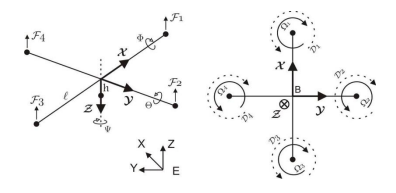
\includegraphics[scale=1]{gambar/quadcopter_koordinat.png}
  % Keterangan gambar yang diinputkan
  \caption{Sistem Koordinat pada Quadcopter}
  % Label referensi dari gambar yang diinputkan
  \label{fig:quad_coordinate}
\end{figure}

Quadcopter dapat terbang dan bergerak dengan cara melakukan pengontrolan gaya angkat dan torsi dengan melakukan pembedaan kecepatan putar keempat motornya. Sebuah quadcopter memiliki 3 \emph{Degree of Freedom} atau DoF yaitu \emph{Yaw}, \emph{Pitch} dan \emph{Roll}. Pergerakan pada DoF ini dilakukan dengan cara mengatur kecepatan putar masing-masing motor sesuai dengan arah gerakan quadcopter. Sementara itu, untuk melakukan terbang secara seimbang, sebuah quadcopter perlu melakukan penyeimbangan kecepatan putaran motor untuk seluruh motornya sehingga diperlukan juga masukan atau input dari sensor sebagai pembanding apakah sebuah quadcopter ini seimbang atau tidak, sensor yang biasa digunakan pada sebuah quadcopter adalah \emph{accelerometer} dan \emph{gyroscope} \cite{PraveenQuadcopter}.

\subsection{Pengolahan Citra}

Pada sebuah komputer modern, citra yang ditemui pada dunia nyata tidak dapat secara langsung direpresentasikan oleh komputer. Dalam merubah bentuk citra di dunia nyata atau yang sering disebut citra analog perlu dilakukan perubahan dengan menggunakan sistem \emph{sampling}. Sistem \emph{sampling} ini berguna untuk mengubah citra analog menjadi M baris N kolom dan hasil ini dapat didefinisikan sebagai citra diskrit. Pertemuan titik antara M baris dan N kolom ini dinamakan dengan Piksel atau titik terkecil dari sebuah citra digital. Selain sistem \emph{sampling}, di dalam citra digital juga terdapat kuantisasi. Kuantitasi adalah sebuah pemberian nilai-nilai tertentu pada sebuah piksel di dalam citra digital. Nilai kuantisasi ini dapat merepresentasikan warna maupun kecerahan dari piksel di dalam sebuah citra digital.

Dengan adanya piksel dan hasil nilai kuantisasi maka dapat dilakukan pengoperasian matematika pada nilai kuantisasi di seluruh piksel yang dimiliki sebuah citra digital. Salah satu cara pengolahan yang paling mudah adalah dengan menggunakan library yang bernama OpenCV \cite{KusumantoPengolahanCitra}. OpenCV mampu membantu dalam pemrosesan data nilai suatu gambar yang dimana di dalam komputer hasil dari \emph{sampling} dan kuantisasi ini direpresentasikan sebagai sebuah array. Pengolahan citra sering digunakan untuk mempersiapakan gambar sebelum diolah oleh program \emph{machine learning} sehingga menghasilkan hasil keputusan yang jauh lebih baik dibandingkan langsung memberikan gambar.

\subsection{\emph{Deep Learning}}

\emph{Deep Learning} adalah sebuah bidang di dalam dunia pembelajaran mesin. Di dalam \emph{Deep Learning} terdapat sebuah konsep yang disebut dengan \emph{Deep Neural Network}, yaitu sebuah gabungan dari beberapa program pembalajaran mesin ataupun model dalam menentukan sebuah keputusan yang menyerupai bagaimana otak manusia dalam mengambil keputusan. Keputusan ini diambil dengan menirukan bagaimana neuron dalam otak manusia melakukan identifikasi fenomena, melakukan penimbangan opsi serta menghasilkan sebuah keputusan atau konklusi \cite{IBMDeepLearning}. 

Di dalam sebuah \emph{Neural Network} terdapat beberapa lapisan node yang mensimulasikan sebuah neuron di otak manusia. Setiap node ini tersambung satu sama lain. Apabila sebuah keluaran dari sebuah node melebihi nilai yang dibatasinya, maka node akan mengeluarkan data ke lapisan berikutnya sehingga mengaktifkan lapisan node berikutnya. Hal ini membuat \emph{Deep Neural Network} sangat cocok digunakan untuk permasalahan yang jauh lebih kompleks dibandingkan pembelajaran mesin tradisional. Dalam penggunaan \emph{Deep Neural Network} diperlukan daya komputer yang jauh lebih kuat dibandingkan pembelajaran mesin tradisional. Hal ini dikarenakan perlu dilakukan banyak perhitungan secara bersamaan dalam mengaktifkan banyak layer. Namun dengan pengembangan \emph{Compute Unit} atau CU khusus untuk pemroses pembelajaran mesin pada GPU (\emph{Graphic Processing Unit}), CPU (\emph{Central Processing Unit}) dan TPU (\emph{Tensor Processing Unit}) pada komputer membuat pengolahan layer secara langsung dan bersamaan semakin mudah dan cepat \cite{Goodfellow-et-al-2016}.

Beberapa pengaplikasian utama dalam \emph{Deep Learning} untuk melakukan pengolahan gambar. Deep learning memungkinkan sebuah komputer untuk mengetahui gambar apa yang sedang diterimanya. \emph{Deep Learning} banyak digunakan oleh robot untuk melakukan pengenalan akan keadaan sekitarnya, contohnya adalah pada mobil otonom yang mampu mendeteksi jalan dengan kameranya. Selain melalui kamera, di mobil otonom juga terdapat \emph{Deep Learning} yang dapat menganalisis data, baik data yang berasal dari berbagai sensor seperti Lidar, GPS, maupun dataset seperti peraturan di jalan, rambu-rambu di jalan, sehingga dapat mengambil keputusan saat melakukan pengendalian otonomnya.

\subsection{YOLO}
YOLO atau \emph{You Only Look Once} adalah sebuah model pendeteksian objek yang paling mutakhir yang dikembangkan oleh Joseph Redmon, Santosh Divvala, Ross Girshick dan Ali Farhadi. YOLO adalah salah satu sistem yang mengimplementasikan \emph{Deep Learning} di dalam ranah pengolahan citra dan video \cite{RedmonYOLO}.
\begin{figure} [H] \centering
  % Nama dari file gambar yang diinputkan
  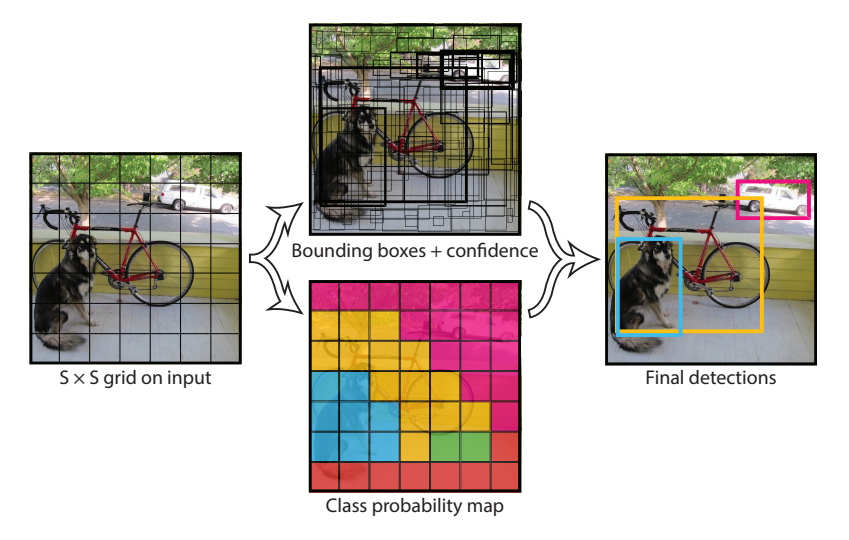
\includegraphics[scale=0.5]{gambar/yolo_method.png}
  % Keterangan gambar yang diinputkan
  \caption{Proses Deteksi pada YOLO}
  % Label referensi dari gambar yang diinputkan
  \label{fig:yolo_detection}
\end{figure}

Pada sistem pendeteksian gambar sebelum YOLO, biasanya sistem bekerja dengan cara melakukan klasifikasi dan lokalisasi model terhadap gambar pada berbagai bagian di gambar dan juga pada berbagai skala, lalu dihasilkan nilai tinggi yang akan diklasifikasikan sebagai terdeteksi. Pada YOLO hal ini dilakukan satu buah pendeteksian ke satu \emph{neural network} secara penuh dan langsung (tanpa dibagi-bagi), kemudian \emph{Neural Network} YOLO akan membagi-bagi gambar menjadi bagian-bagian dan memprediksi bagian-bagian ini untuk diberikan batasan dan probabilitas. Batasan-batasan inilah yang kemudian akan ditimbang nilainya berdasarkan prediksi probabilitasnya. Dikarenakan penggunaan pendeteksian langsung ke seluruh gambar di awal membuat YOLO menjadi jauh lebih cepat dibandingkan dengan menggunakan sistem \emph{machine learning} tradisional seperti R-CNN atau bahkan Fast R-CNN. 


% \subsection{\emph{Optical Flow}}

% \subsection{\emph{Real Time Protocol}}

\subsection{\emph{Quality of Service} (QoS)}

QoS atau \emph{Quality of Service} adalah sebuah mekanisme dalam teknologi jaringan dimana dilakukan pengontrolan pada pengiriman data melalui jaringan untuk memastikan bahwa aplikasi atau hal penting yang ingin dilakukan melalui suatu jaringan tidak terputus atau terganggu walaupun dengan kapasitas jaringan yang kecil. Dengan adanya QoS, maka di dalam suatu sistem dapat diprioritaskan data apa yang harus selalu terkirim secara penuh dan tidak pernah menghilang atau terputus. Hal ini membuat ketika QoS digunakan maka suatu sistem dapat diatur seberapa \emph{bandwidth} data yang digunakan saat transmissi melalui jaringan dan seberapa lama data akan sampai ke ujung lainnya dari jaringan tersebut. Salah satu pengaplikasian QoS adalah di dalam gedung perusahaan pengiriman gambar video CCTV ke ruang server akan diprioritaskan dibandingkan data lain, dikarenakan ini berkaitan dengan keamanan gedung.

Cara kerja QoS adalah dengan memberikan penanda pada paket data yang dikirimkan oleh sebuah aplikasi, dan kemudian membuat jalur khusus pada router untuk setiap aplikasi. Hal ini membuat setiap aplikasi dan data yang dimilikinya memiliki prioritas yang berbeda-beda satu dengan yang lain. Hal ini membuat \emph{bandwidth} untuk aplikasi dengan prioritas tinggi atau yang krusial akan pasti selalu tersedia. Selain itu QoS juga juga mengatur bagaimana suatu jaringan membagi \emph{resource} dan bagaimana dia mengontrol alokasi jalur pada suatu jaringan. Beberapa hal yang diperhatikan di dalam QoS adalah sebagai berikut :
\begin{enumerate}
  \item \emph{Bandwidth} : berapa banyak jumlah data yang dikirim dalam periode waktu (bps).
  \item \emph{Delay} : waktu yang diperlukan dari saat paket data dikirimkan dan diterima (ms).
  \item \emph{Loss} : persentase data yang hilang saat pengiriman.
  \item \emph{Jitter} : perubahaan kecepatan yang terjadi di jaringan akibat macetnya transfer data.
\end{enumerate}
Keuntungan dari penggunaan QoS pada suatu jaringan adalah sebagai berikut :
\begin{enumerate}
  \item Penjaminan akan terus berjalanan aplikasi yang krusial atau penting pada jaringan.
  \item Pengelolaan sumber daya internet yang bagus.
  \item Penanggulangan hilangnya data.
  \item Pengurangan latensi atau keterlambatan jaringan.
  
\end{enumerate}

% \subsection{Hukum Newton}

% % Contoh penggunaan referensi dari persamaan
% Kemudian menjadi persamaan seperti pada persamaan \ref{eq:FirstLaw}.

% % Contoh pembuatan persamaan
% \begin{equation}
%   % Label referensi dari persamaan yang dibuat
%   \label{eq:FirstLaw}
%   % Baris kode persamaan yang dibuat
%   \sum \mathbf{F} = 0\; \Leftrightarrow\; \frac{\mathrm{d} \mathbf{v} }{\mathrm{d}t} = 0.
% \end{equation}
  \cleardoublepage

  % Konten metodologi
  \chapter{METODOLOGI}

% Ubah konten-konten berikut sesuai dengan isi dari metodologi

\section{Metode yang digunakan}

\lipsum[11]

% Contoh input gambar dengan format *.jpg
\begin{figure} [H] \centering
  % Nama dari file gambar yang diinputkan
  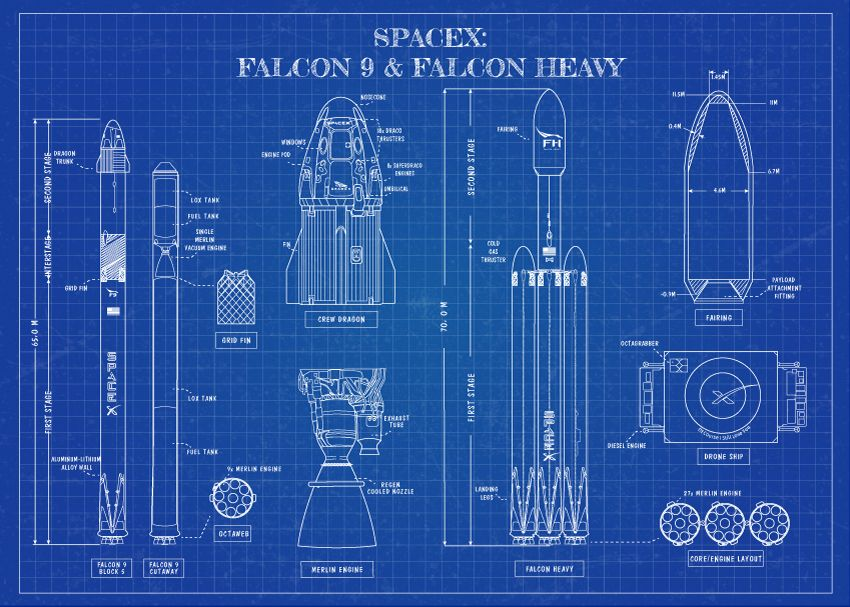
\includegraphics[scale=0.45]{gambar/blueprint.jpg}
  % Keterangan gambar yang diinputkan
  \caption{\emph{Blueprint} roket yang akan diuji coba \parencite{SpaceXBlueprint}}
  % Label referensi dari gambar yang diinputkan
  \label{fig:Blueprint}
\end{figure}

% Contoh penggunaan referensi dari gambar yang diinputkan
Pada \emph{blueprint} yang tertera di Gambar \ref{fig:Blueprint}. \lipsum[12]

\section{Bahan dan peralatan yang digunakan}

\lipsum[13]

  \cleardoublepage

  % Konten lainnya
  \chapter{HASIL YANG DIHARAPKAN}

\section{Hasil yang Diharapkan dari Penelitian}

Hasil yang diharapkan dari penelitian ini adalah suatu sistem \emph{monitoring} yang fleksibel menggunakan teknologi drone. Dimana sistem \emph{monitoring} ini dapat memantau antrian kendaraan yang ada pada daerah lalu lintas dengan akurat. selain itu, dengan dilakukannya penelitian ini diharapkan dapat berkontribusi dalam mengatasi masalah kemacetan yang terjadi saat ini. Penelitian ini juga bisa membantu pengembangan konsep \emph{smart city}, karena data antrian yang dihasilkan bisa bermanfaat pada sistem lalu lintas yang cerdas di lingkungan \emph{smart city}.

\section{Hasil Pendahuluan}

Sampai saat ini, penulis telah mencoba mengimplementasikan model YOLO untuk mendeteksi kendaraan pada suatu lalu lintas. Versi YOLO yang dipakai adalah YOLOv5. Dataset yang digunakan berasal dari VisDrone, yaitu sebuah dataset yang dirancang khusus untuk penelitian dalam bidang visi komputer yang berfokus pada analisis video dan gambar yang diambil dari drone.

Awalnya penulis mencoba menggunakan model dengan hasil training dari dataset yang sudah jadi yaitu COCO (Common Object in Context), dan saat dilakukan deteksi kendaran mendapatkan hasil berikut.
\begin{figure} [H] \centering
    % Nama dari file gambar yang diinputkan
    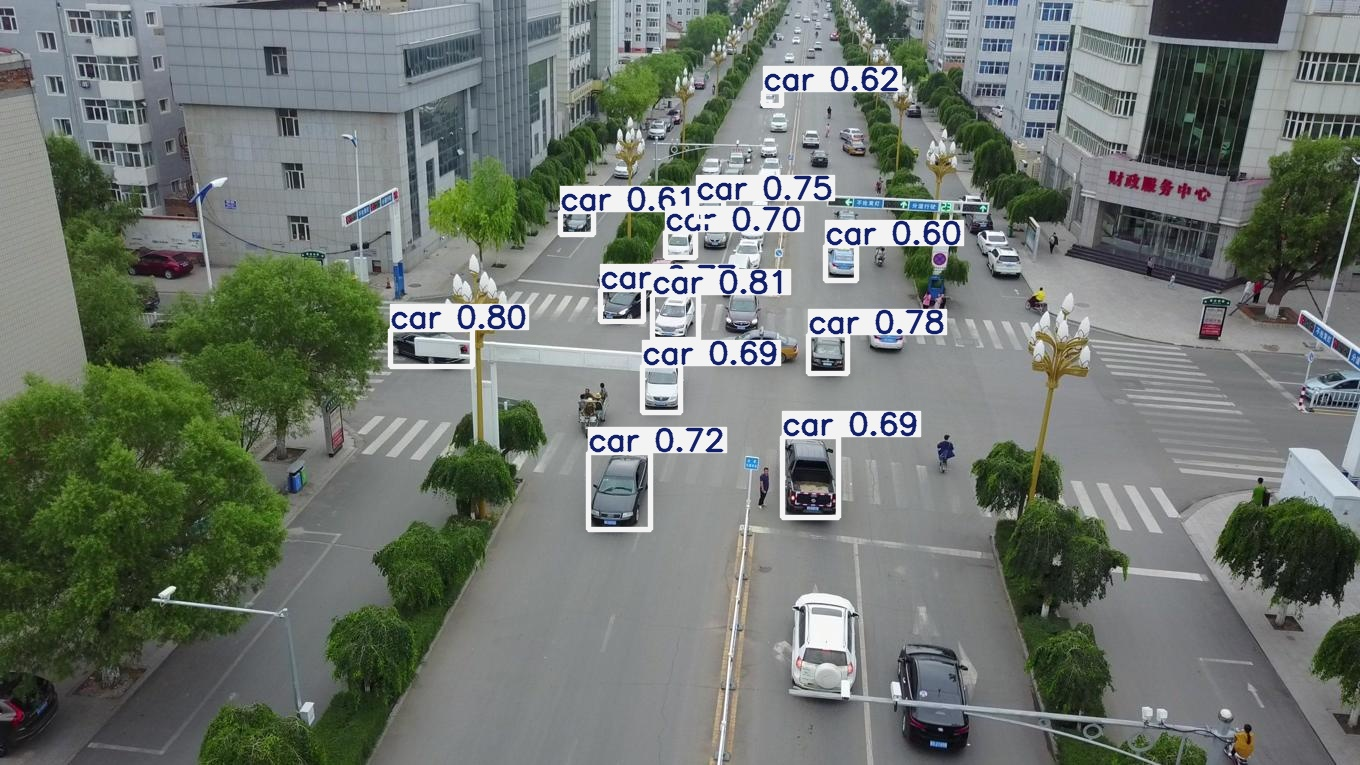
\includegraphics[scale=0.3]{gambar/coco_1.jpg}
    % Keterangan gambar yang diinputkan
    \caption{Proses Deteksi dengan dataset COCO}
    % Label referensi dari gambar yang diinputkan
    \label{fig:deteksi_kendaraan_coco1}
  \end{figure}
  
  Namun, pada implementasinya nanti posisi kamera seharusnya tidak seperti pada gambar \ref{fig:deteksi_kendaraan_coco1}, sehingga dicoba dilakukan deteksi dengan sudut pandang lain yang lebih sesuai. 
  \begin{figure} [H] \centering
      % Nama dari file gambar yang diinputkan
      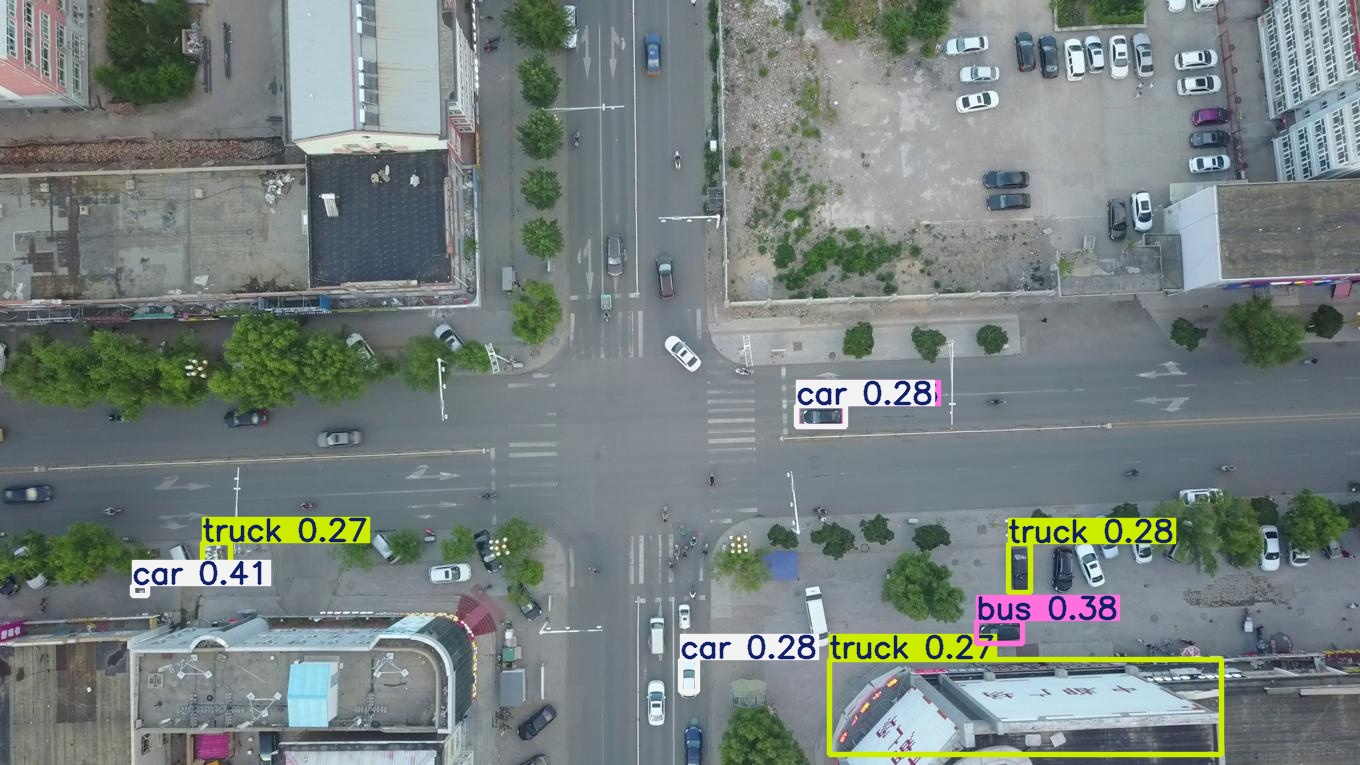
\includegraphics[scale=0.3]{gambar/coco_2.jpg}
      % Keterangan gambar yang diinputkan
      \caption{Proses Deteksi dengan dataset COCO dengan \emph{angle} lebih sesuai}
      % Label referensi dari gambar yang diinputkan
      \label{fig:deteksi_kendaraan_coco2}
    \end{figure}
    
Dikarenakan dataset COCO yang kurang sesuai dengan pengaplikasian yang dimaksudkan pad penelitian ini, penulis mencoba melakukan trainig dengan dataset VisDrone. Penulis melalui proses \emph{labelling}, \emph{pre-processing}, hingga \emph{training} sesuai keterangan di bab 3 Metodologi. Hasil dari model yang di training tersebut seperti berikut.
\begin{figure} [H] \centering
    % Nama dari file gambar yang diinputkan
    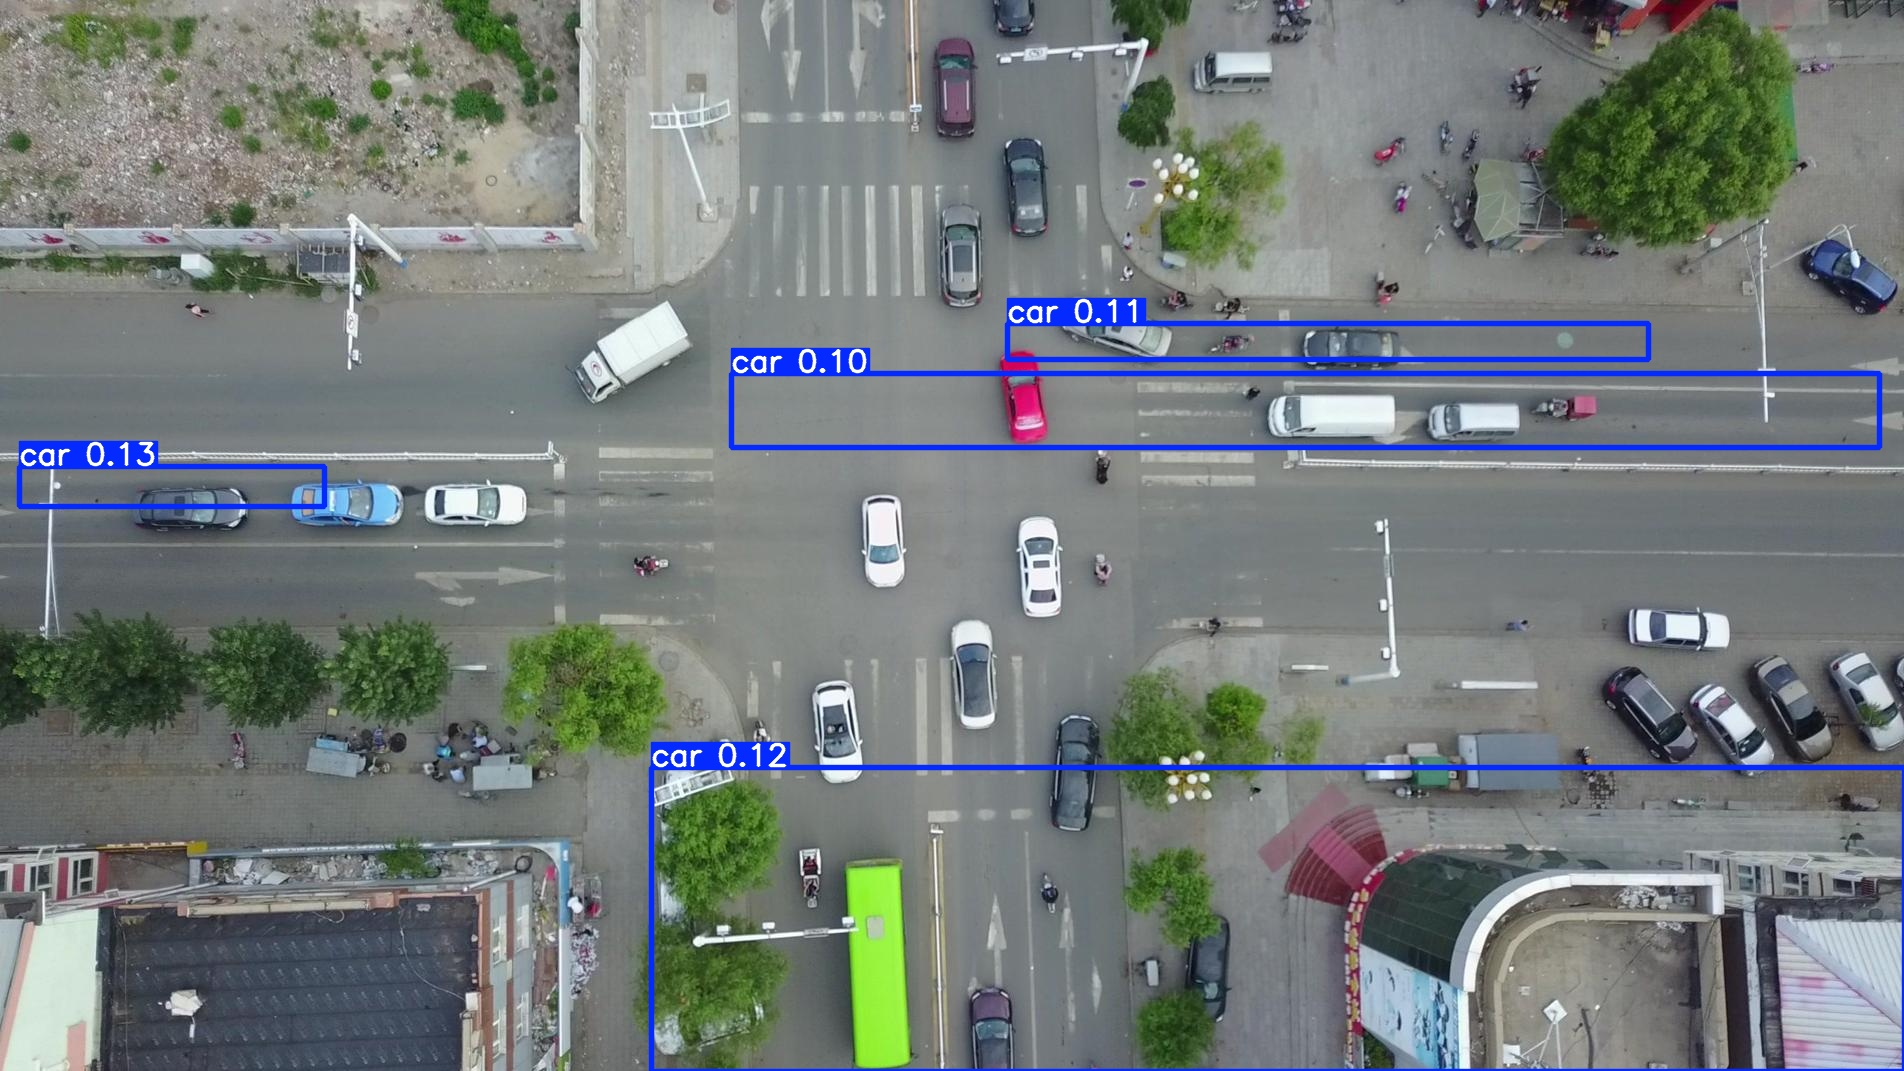
\includegraphics[scale=0.2]{gambar/custom_model.jpg}
    % Keterangan gambar yang diinputkan
    \caption{Proses Deteksi dengan dataset VisDrone}
    % Label referensi dari gambar yang diinputkan
    \label{fig:deteksi_kendaraan_visdrone}
    \end{figure}

Performa yang didapatkan masih belum memenuhi kebutuhan penelitian. Evaluasi dan koreksi harus dilakukan untuk mendapatkan performa model yang diinginkan sesuai dengan kebutuhan penelitian. Meskipun demikian, penulis berkomitmen untuk meneruskan prosedur yang sudah direncanakan agar penelitian ini dapat berjalan sesuai rencana.
  \cleardoublepage

  % \chapter{JADWAL PENELITIAN}

% Ubah tabel berikut sesuai dengan isi dari rencana kerja
\newcommand{\w}{}
\newcommand{\G}{\cellcolor{gray}}
\begin{table}[H]
  \captionof{table}{Tabel timeline}
  \label{tbl:timeline}
  \begin{tabular}{|p{3.5cm}|c|c|c|c|c|c|c|c|c|c|c|c|c|c|c|c|}

    \hline
    \multirow{2}{*}{Kegiatan} & \multicolumn{16}{|c|}{Minggu}                                                                       \\
    \cline{2-17}              &
    1                         & 2                             & 3  & 4  & 5  & 6  & 7  & 8  & 9  & 10 & 11 & 12 & 13 & 14 & 15 & 16 \\
    \hline

    % Gunakan \G untuk mengisi sel dan \w untuk mengosongkan sel
    Pengambilan data          &
    \G                        & \G                            & \G & \G & \w & \w & \w & \w & \w & \w & \w & \w & \w & \w & \w & \w \\
    \hline

    Pengolahan data           &
    \w                        & \w                            & \w & \w & \G & \G & \G & \G & \w & \w & \w & \w & \w & \w & \w & \w \\
    \hline

    Analisa data              &
    \w                        & \w                            & \w & \w & \w & \w & \w & \w & \G & \G & \G & \G & \w & \w & \w & \w \\
    \hline

    Evaluasi penelitian       &
    \w                        & \w                            & \w & \w & \w & \w & \w & \w & \w & \w & \w & \w & \G & \G & \G & \G \\
    \hline
  \end{tabular}
\end{table}

Pada \emph{timeline} yang tertera di Tabel \ref{tbl:timeline} \lipsum[10]

  % \cleardoublepage

  % Daftar pustaka
  \chapter*{DAFTAR PUSTAKA}
  \addcontentsline{toc}{chapter}{DAFTAR PUSTAKA}
  \renewcommand\refname{}
  \vspace{2ex}
  \renewcommand{\bibname}{}
  \begingroup
    \def\chapter*#1{}
    \printbibliography
  \endgroup


\end{document}
